\documentclass[journal,12pt,twocolumn]{IEEEtran}
%
\usepackage{setspace}
\usepackage{multicol}
\usepackage{gensymb}
\usepackage{enumerate}
\usepackage{xcolor}
\usepackage{caption}
%\usepackage{subcaption}
%\doublespacing
\singlespacing

%\usepackage{graphicx}
%\usepackage{amssymb}
%\usepackage{relsize}
\usepackage[cmex10]{amsmath}
\usepackage{mathtools}
%\usepackage{amsthm}
%\interdisplaylinepenalty=2500
%\savesymbol{iint}
%\usepackage{txfonts}
%\restoresymbol{TXF}{iint}
%\usepackage{wasysym}
\usepackage{amsthm}
\usepackage{mathrsfs}
\usepackage{txfonts}
\usepackage{stfloats}
\usepackage{cite}
\usepackage{cases}
\usepackage{subfig}
%\usepackage{xtab}
\usepackage{longtable}
\usepackage{multirow}
%\usepackage{algorithm}
%\usepackage{algpseudocode}
%\usepackage{enumitem}
\usepackage{mathtools}
\usepackage{iithtlc}
%\usepackage[framemethod=tikz]{mdframed}
\usepackage{listings}


%\usepackage{stmaryrd}


%\usepackage{wasysym}
%\newcounter{MYtempeqncnt}
\DeclareMathOperator*{\Res}{Res}
%\renewcommand{\baselinestretch}{2}
\renewcommand\thesection{\arabic{section}}
\renewcommand\thesubsection{\thesection.\arabic{subsection}}
\renewcommand\thesubsubsection{\thesubsection.\arabic{subsubsection}}

\renewcommand\thesectiondis{\arabic{section}}
\renewcommand\thesubsectiondis{\thesectiondis.\arabic{subsection}}
\renewcommand\thesubsubsectiondis{\thesubsectiondis.\arabic{subsubsection}}

% correct bad hyphenation here
\hyphenation{op-tical net-works semi-conduc-tor}

\lstset{
language=Python,
frame=single, 
breaklines=true
}

%\lstset{
	%%basicstyle=\small\ttfamily\bfseries,
	%%numberstyle=\small\ttfamily,
	%language=python,
	%backgroundcolor=\color{white},
	%%frame=single,
	%%keywordstyle=\bfseries,
	%%breaklines=true,
	%%showstringspaces=false,
	%%xleftmargin=-10mm,
	%%aboveskip=-1mm,
	%%belowskip=0mm
%}

%\surroundwithmdframed[width=\columnwidth]{lstlisting}


\begin{document}
%

\theoremstyle{definition}
\newtheorem{theorem}{Theorem}[section]
%\newtheorem{problem}{Problem}[section]
\newtheorem{problem}{Problem}
\newtheorem{proposition}{Proposition}
%\newtheorem{proposition}{Proposition}[section]
\newtheorem{lemma}{Lemma}[section]
\newtheorem{corollary}[theorem]{Corollary}
\newtheorem{example}{Example}[section]
%\newtheorem{definition}{Definition}[section]
\newtheorem{definition}{Definition}
%\newtheorem{definition}{Definition}
%\newtheorem{algorithm}{Algorithm}[section]
%\newtheorem{cor}{Corollary}
\newcommand{\BEQA}{\begin{eqnarray}}
\newcommand{\EEQA}{\end{eqnarray}}
\newcommand{\define}{\stackrel{\triangle}{=}}

\bibliographystyle{IEEEtran}
%\bibliographystyle{ieeetr}

\providecommand{\nCr}[2]{\,^{#1}C_{#2}} % nCr
\providecommand{\nPr}[2]{\,^{#1}P_{#2}} % nPr
\providecommand{\mbf}{\mathbf}
\providecommand{\pr}[1]{\ensuremath{\Pr\left(#1\right)}}
\providecommand{\qfunc}[1]{\ensuremath{Q\left(#1\right)}}
\providecommand{\sbrak}[1]{\ensuremath{{}\left[#1\right]}}
\providecommand{\lsbrak}[1]{\ensuremath{{}\left[#1\right.}}
\providecommand{\rsbrak}[1]{\ensuremath{{}\left.#1\right]}}
\providecommand{\brak}[1]{\ensuremath{\left(#1\right)}}
\providecommand{\lbrak}[1]{\ensuremath{\left(#1\right.}}
\providecommand{\rbrak}[1]{\ensuremath{\left.#1\right)}}
\providecommand{\cbrak}[1]{\ensuremath{\left\{#1\right\}}}
\providecommand{\lcbrak}[1]{\ensuremath{\left\{#1\right.}}
\providecommand{\rcbrak}[1]{\ensuremath{\left.#1\right\}}}
\theoremstyle{remark}
\newtheorem{rem}{Remark}
\newcommand{\sgn}{\mathop{\mathrm{sgn}}}
\providecommand{\abs}[1]{\left\vert#1\right\vert}
\providecommand{\res}[1]{\Res\displaylimits_{#1}} 
\providecommand{\norm}[1]{\lVert#1\rVert}
\providecommand{\mtx}[1]{\mathbf{#1}}
\providecommand{\mean}[1]{E\left[ #1 \right]}
\providecommand{\fourier}{\overset{\mathcal{F}}{ \rightleftharpoons}}
%\providecommand{\hilbert}{\overset{\mathcal{H}}{ \rightleftharpoons}}
\providecommand{\system}{\overset{\mathcal{H}}{ \longleftrightarrow}}
	%\newcommand{\solution}[2]{\textbf{Solution:}{#1}}
\newcommand{\solution}{\noindent \textbf{Solution: }}
\providecommand{\dec}[2]{\ensuremath{\overset{#1}{\underset{#2}{\gtrless}}}}
\numberwithin{equation}{section}
%\numberwithin{equation}{problem}
%\numberwithin{problem}{subsection}
%\numberwithin{definition}{subsection}
\makeatletter
\@addtoreset{figure}{problem}
\makeatother

\let\StandardTheFigure\thefigure
%\renewcommand{\thefigure}{\theproblem.\arabic{figure}}
\renewcommand{\thefigure}{\theproblem}


%\numberwithin{figure}{subsection}

\def\putbox#1#2#3{\makebox[0in][l]{\makebox[#1][l]{}\raisebox{\baselineskip}[0in][0in]{\raisebox{#2}[0in][0in]{#3}}}}
     \def\rightbox#1{\makebox[0in][r]{#1}}
     \def\centbox#1{\makebox[0in]{#1}}
     \def\topbox#1{\raisebox{-\baselineskip}[0in][0in]{#1}}
     \def\midbox#1{\raisebox{-0.5\baselineskip}[0in][0in]{#1}}

\vspace{3cm}

\title{ 
\logo{
Series
}
%	\logo{python for Math Computing }
}
%\title{
%	\logo{Matrix Analysis through python}{\begin{center}\includegraphics[scale=.24]{tlc}\end{center}}{}{HAMDSP}
%}


% paper title
% can use linebreaks \\ within to get better formatting as desired
%\title{Matrix Analysis through python}
%
%
% author names and IEEE memberships
% note positions of commas and nonbreaking spaces ( ~ ) LaTeX will not break
% a structure at a ~ so this keeps an author's name from being broken across
% two lines.
% use \thanks{} to gain access to the first footnote area
% a separate \thanks must be used for each paragraph as LaTeX2e's \thanks
% was not built to handle multiple paragraphs
%

\author{P.~N.~V.~S.~S.~K.~ HAVISH$^{*}$, S.~.S.~Ashish$^{*}$, J.~Balasubramaniam$^{\dagger}$ and G V V Sharma$^{*}$ %<-this  stops a space
\thanks{$\dagger$ The author is with the Department of Mathematics, IIT Hyderabad.  *The authors are with the Department
of Electrical Engineering, IIT, Hyderabad
502285 India e-mail: \{ee16btech11023,ee16btech11043,jbala,gadepall\}@iith.ac.in. All material in the manuscript is released under GNU GPL.  Free to use for all.}% <-this % stops a space
%\thanks{J. Doe and J. Doe are with Anonymous University.}% <-this % stops a space
%\thanks{Manuscript received April 19, 2005; revised January 11, 2007.}}
}
% note the % following the last \IEEEmembership and also \thanks - 
% these prevent an unwanted space from occurring between the last author name
% and the end of the author line. i.e., if you had this:
% 
% \author{....lastname \thanks{...} \thanks{...} }
%                     ^------------^------------^----Do not want these spaces!
%
% a space would be appended to the last name and could cause every name on that
% line to be shifted left slightly. This is one of those "LaTeX things". For
% instance, "\textbf{A} \textbf{B}" will typeset as "A B" not "AB". To get
% "AB" then you have to do: "\textbf{A}\textbf{B}"
% \thanks is no different in this regard, so shield the last } of each \thanks
% that ends a line with a % and do not let a space in before the next \thanks.
% Spaces after \IEEEmembership other than the last one are OK (and needed) as
% you are supposed to have spaces between the names. For what it is worth,
% this is a minor point as most people would not even notice if the said evil
% space somehow managed to creep in.



% The paper headers
%\markboth{Journal of \LaTeX\ Class Files,~Vol.~6, No.~1, January~2007}%
%{Shell \MakeLowercase{\textit{et al.}}: Bare Demo of IEEEtran.cls for Journals}
% The only time the second header will appear is for the odd numbered pages
% after the title page when using the twoside option.
% 
% *** Note that you probably will NOT want to include the author's ***
% *** name in the headers of peer review papers.                   ***
% You can use \ifCLASSOPTIONpeerreview for conditional compilation here if
% you desire.




% If you want to put a publisher's ID mark on the page you can do it like
% this:
%\IEEEpubid{0000--0000/00\$00.00~\copyright~2007 IEEE}
% Remember, if you use this you must call \IEEEpubidadjcol in the second
% column for its text to clear the IEEEpubid mark.



% make the title area
\maketitle

%\newpage

%\tableofcontents


%\begin{abstract}
%%\boldmath
%In this letter, an algorithm for evaluating the exact analytical bit error rate  (BER)  for the piecewise linear (PL) combiner for  multiple relays is presented. Previous results were available only for upto three relays. The algorithm is unique in the sense that  the actual mathematical expressions, that are prohibitively large, need not be explicitly obtained. The diversity gain due to multiple relays is shown through plots of the analytical BER, well supported by simulations. 
%
%\end{abstract}
% IEEEtran.cls defaults to using nonbold math in the Abstract.
% This preserves the distinction between vectors and scalars. However,
% if the journal you are submitting to favors bold math in the abstract,
% then you can use LaTeX's standard command \boldmath at the very start
% of the abstract to achieve this. Many IEEE journals frown on math
% in the abstract anyway.

% Note that keywords are not normally used for peerreview papers.
%\begin{IEEEkeywords}
%Cooperative diversity, decode and forward, piecewise linear
%\end{IEEEkeywords}



% For peer review papers, you can put extra information on the cover
% page as needed:
% \ifCLASSOPTIONpeerreview
% \begin{center} \bfseries EDICS Category: 3-BBND \end{center}
% \fi
%
% For peerreview papers, this IEEEtran command inserts a page break and
% creates the second title. It will be ignored for other modes.
\IEEEpeerreviewmaketitle

\bigskip

\begin{abstract}
This manual covers the convergence/divergence of series through examples.  Python scripts are provided for understanding the propagation of the series.
\end{abstract}
%

%\section{Limit}
\begin{problem}
\label{prob:ratio}
Sketch the series whose $n$th term is 
\begin{equation}
\label{eq:ratio}
u_{n}=\brak{\frac{1}{\sqrt{2}}}^{n}
\end{equation}
\end{problem}
%
\solution
%\input{./problems/ee16b1001.tex}
\lstinputlisting{./codes/1.py}
%
\begin{figure}[!ht]
\begin{center}
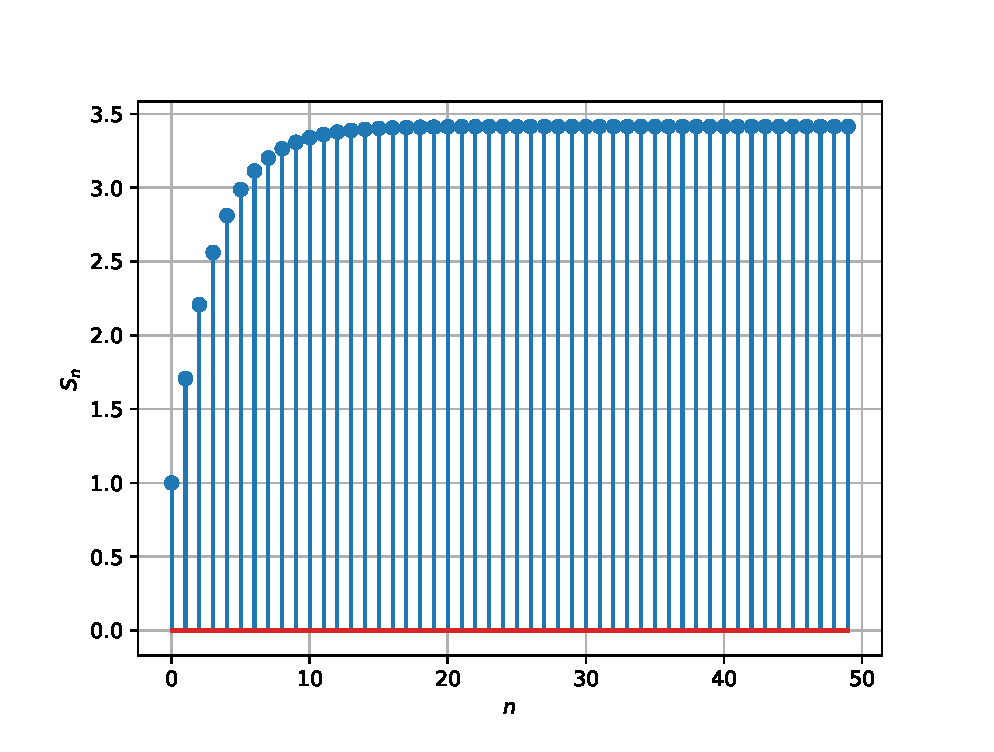
\includegraphics[width=\columnwidth]{./figs/1.eps}
\end{center}
\captionof{figure}{}

\label{fig:1}	
\end{figure}
%
\begin{proposition}
\label{prop:root_test}
%
({\em Root test}) If
\begin{align}
\lim_{n\rightarrow \infty}u_n^{\frac{1}{n}} < 1
\end{align}
%
then the series defined by
\begin{equation}
S_n = \sum_{k=1}^{n}u_k
\end{equation}
converges.
\end{proposition}
\begin{problem}
Show that the series in Problem \ref{prob:ratio} converges using the root test.
\end{problem}
\begin{proposition}
\label{prop:ratio}
({\em Ratio test})If 
\begin{align}
\lim_{n\rightarrow \infty}\abs{\frac{u_{n+1}}{u_n}}< 1,
\end{align}
then $S_n$ converges.
\end{proposition}
\begin{problem}
Show that the series in Problem \ref{prob:ratio} converges using the ratio test.
\end{problem}
%
\begin{problem}
Graphically examine the series 
\begin{equation}
u_{n}=\sqrt{n+1}-\sqrt{n}
\end{equation}

\end{problem}
\solution From Fig. \ref{fig:3}, it can be seen that the series diverges
%\input{./problems/ee16b1001.tex}
\lstinputlisting{./codes/3.py}
%
\begin{figure}[!ht]
\begin{center}
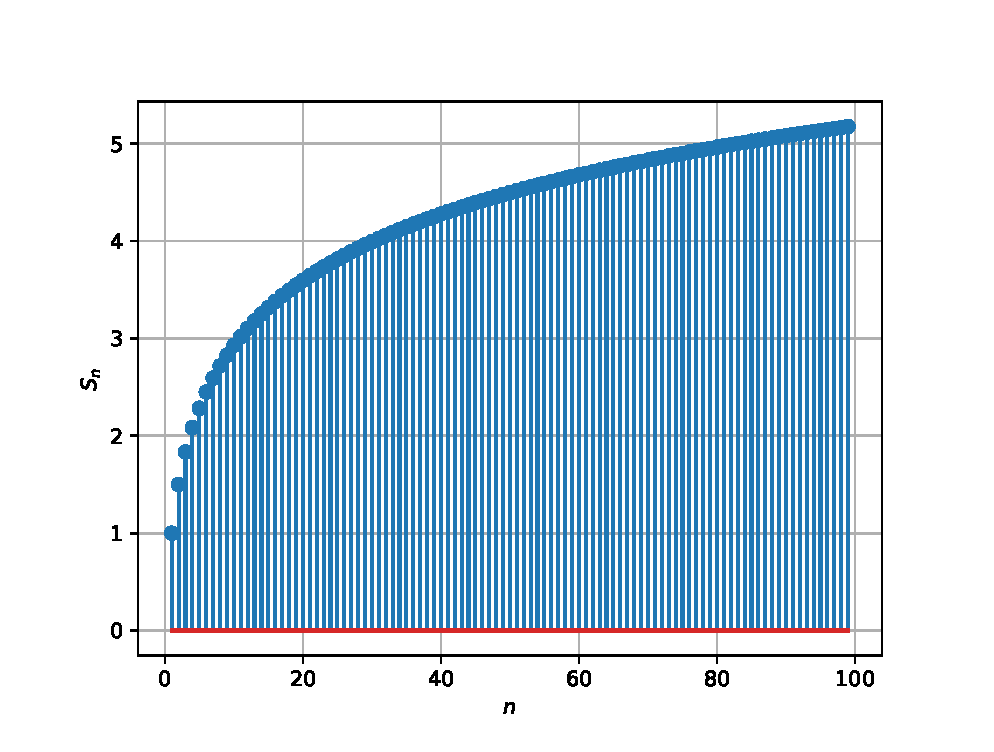
\includegraphics[width=\columnwidth]{./figs/2.eps}
\end{center}
\captionof{figure}{}
\label{fig:3}	
\end{figure}

\begin{problem}
Show that the series defined by 
\begin{equation}
u_{n}=\sqrt{n+1}-\sqrt{n}
\end{equation}
diverges.
\end{problem}
\begin{proof}
Since
\begin{align}
S_n = \sum_{i=1}^{n}u_k = \sqrt{n+1}-1,
\end{align}
which is monotonically increasing as well as unbounded, $S_n$ diverges.
\end{proof}
%
\begin{proposition}
\label{prop:inequality}
Let the $n$th terms of two series be $a_n$ and $b_n$.  If $a_n < b_n$
\begin{enumerate}
\item  and the $b_n$ series converges, then the $a_n$ series also converges.
\item  and the $a_n$ series diverges, then the $b_n$ series diverges.
\end{enumerate}
\end{proposition}
\begin{problem}
\label{prob:inequality}
Sketch the series defined by 
\begin{equation}
u_{n}=\frac{2^n-1}{3^n}
\end{equation}
\end{problem}
%
\solution From Fig. \ref{fig:5}, it can be seen that the series converges.
%\input{./problems/ee16b1001.tex}
\lstinputlisting{./codes/5.py}
%
\begin{figure}[!ht]
\begin{center}
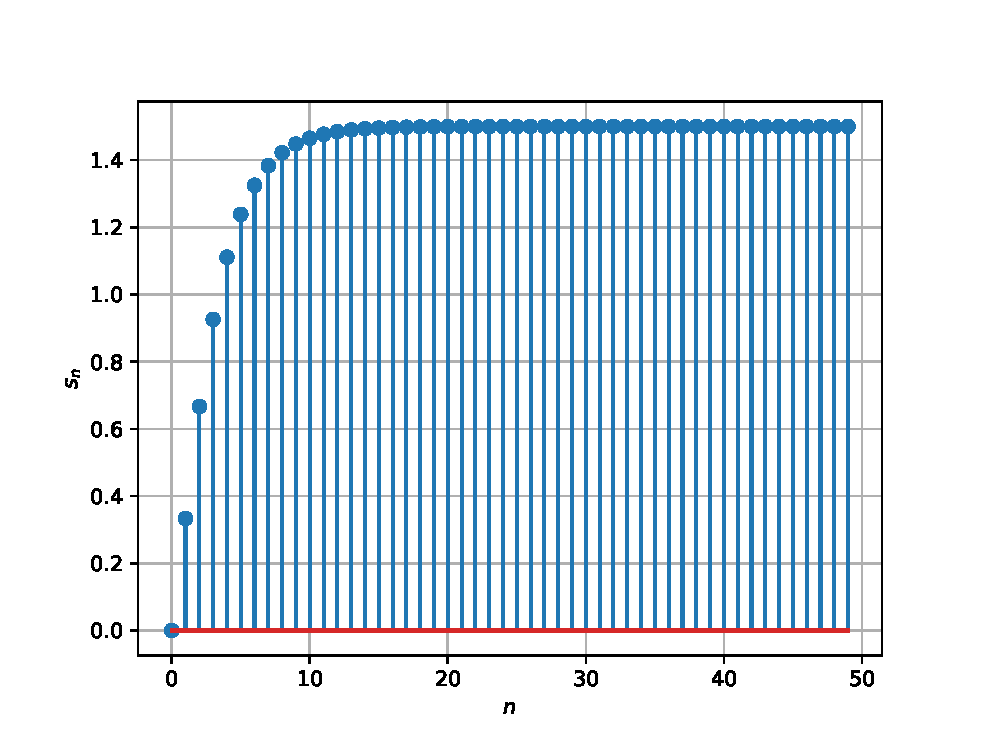
\includegraphics[width=\columnwidth]{./figs/5.eps}
\end{center}
\captionof{figure}{}
\label{fig:5}	
\end{figure}

%

\begin{problem}
Show that $S_n$ in Problem \ref{prob:inequality} converges.
\end{problem}
\solution Since
\begin{align}
u_{n}=\frac{2^n-1}{3^n} < \frac{2^n}{3^n},
\end{align}
using the root test, the $\frac{2^n}{3^n}$ series converges and from Proposition \ref{prop:inequality}, $S_n$ converges.

\begin{proposition}
If $u_n$ is nonnegative and nonincreasing, then $S_n$ converges if and only if the $2^nu_{2^n}$ series converges.
\end{proposition}
\begin{problem}
Graphically examine the series 
\begin{equation}
u_{n}=\frac{1}{n\sqrt{n+1}}
\end{equation}
\end{problem}
\solution From Fig. \ref{fig:6}, it can be seen that the series converges.
%\input{./problems/ee16b1001.tex}
\lstinputlisting{./codes/6.py}
%
\begin{figure}[!ht]
\begin{center}
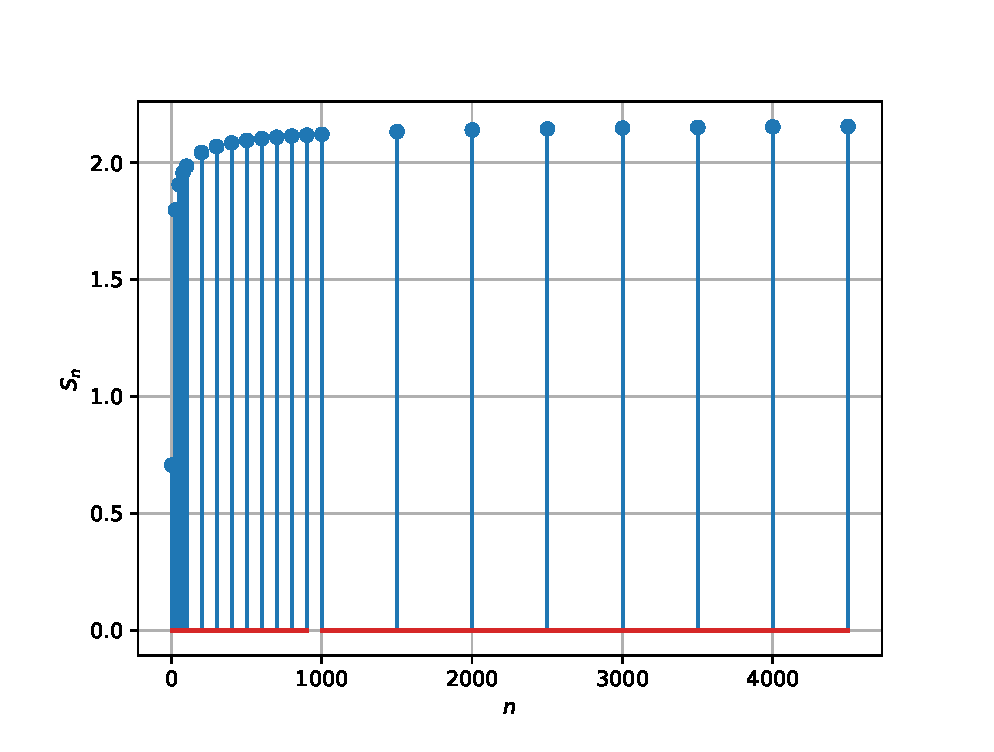
\includegraphics[width=\columnwidth]{./figs/6.eps}
\end{center}
\captionof{figure}{}
\label{fig:6}	
\end{figure}

%
\begin{problem}
Show that 
\begin{equation}
u_{n}=\frac{1}{n\sqrt{n+1}}
\end{equation}
converges.
\end{problem}
\solution It is obvious that
\begin{equation}
u_n =\frac{1}{n\sqrt{n+1}} < \frac{1}{n\sqrt{n}} = f(n), \text{ say }
\end{equation}
Then,
\begin{align}
2^nf(2^n)&= \frac{2^n}{2^{\frac{3n}{2}}}
\\
&= \frac{1}{\brak{\sqrt{2}}^n}
\end{align}
which yields a convergent series using the root test. From Proposition \ref{prop:inequality}, it is obvious that $S_n$ converges.
\begin{proposition}
\label{prop:nonzero}
$S_n$ diverges if $\lim_{n\rightarrow \infty}u_n \ne 0$.
\end{proposition}
\begin{problem}
Graphically examine the series 
\begin{equation}
u_n = \frac{n}{n+1}
\end{equation}
\end{problem}
\solution From Fig. \ref{fig:4}, it can be seen that the series diverges.
%\input{./problems/ee16b1001.tex}
\lstinputlisting{./codes/4.py}
%
\begin{figure}[!ht]
\begin{center}
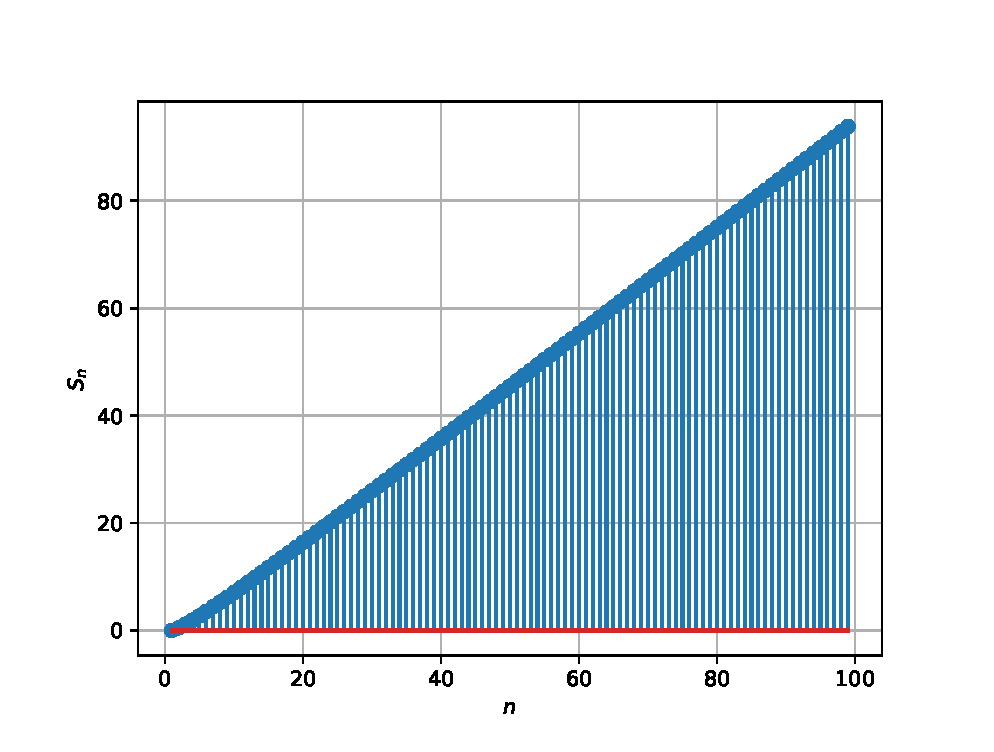
\includegraphics[width=\columnwidth]{./figs/4.eps}
\end{center}
\captionof{figure}{}
\label{fig:4}	
\end{figure}

\begin{problem}
Show that 
\begin{equation}
u_n = \frac{n}{n+1}
\end{equation}
series diverges.
\end{problem}
\begin{proof}
Trivial using Propostion \ref{prop:nonzero}.
\end{proof}
\begin{proposition}
({\em Integral test}) Let $f(n)=u_n$ be positive and monotone decreasing. Then $S_n$ converges if
\begin{equation}
\lim_{t \rightarrow \infty}\int_{1}^{t}f(t)\, dt < \infty
\end{equation}
If the integral diverges, then $S_n$ also diverges.
\end{proposition}
%
\begin{problem}
Graphically examine the series 
\begin{equation}
u_n = \frac{1}{n}
\end{equation}

\end{problem}
\solution From Fig. \ref{fig:2}, it can be seen that the series diverges.
%\input{./problems/ee16b1001.tex}
\lstinputlisting{./codes/2.py}
%
\begin{figure}[!ht]
\begin{center}
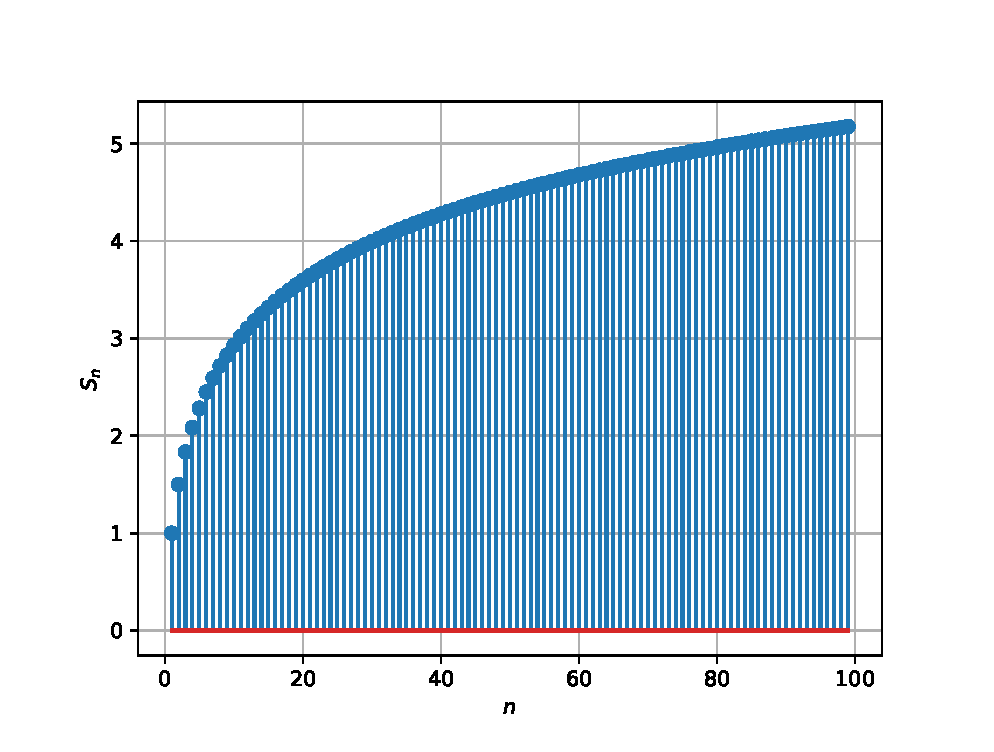
\includegraphics[width=\columnwidth]{./figs/2.eps}
\end{center}
\captionof{figure}{}
\label{fig:2}	
\end{figure}
\begin{problem}
Show that 
\begin{equation}
u_n = \frac{1}{n}
\end{equation}
series diverges.
\end{problem}
\begin{proof}
Using the integral test,
\begin{align}
\lim_{t \rightarrow \infty}\int_{1}^{t}\frac{1}{t}\, dt = \lim_{t \infty}\ln t
\end{align}
which does not converge.  Hence the series diverges.
\end{proof}
\begin{proposition}
\label{prop:leibniz}
({\em Leibniz Test}) If
\begin{equation}
u_n = (-1)^na_n,
\end{equation}
then $S_n$ converges if
\begin{enumerate}
\item $a_n$ is monotonically decreasing
\item $\lim_{n\rightarrow \infty} a_n = 0$
\end{enumerate}
\end{proposition}
%
\begin{problem}
\label{prob:leibniz}
Graphically examine the series 
\begin{equation}
u_n = \frac{\cos n\pi}{\sqrt{n}}
\end{equation}
\end{problem}
\solution From Fig. \ref{fig:7}, it can be seen that the series converges.
%\input{./problems/ee16b1001.tex}
\lstinputlisting{./codes/7.py}
%
\begin{figure}[!ht]
\begin{center}
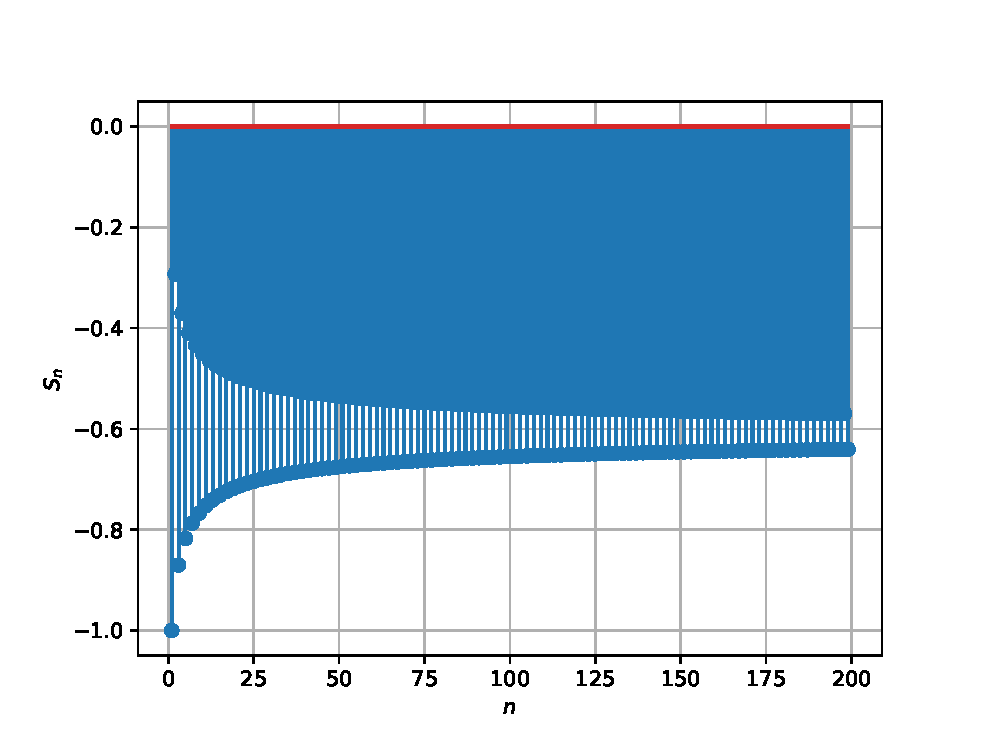
\includegraphics[width=\columnwidth]{./figs/7.eps}
\end{center}
\captionof{figure}{}
\label{fig:7}	
\end{figure}

\begin{problem}
Show that 
\begin{equation}
u_n = \frac{\cos n\pi}{\sqrt{n}}
\end{equation}
converges.
\end{problem}
\begin{proof}
$\frac{1}{\sqrt{n}}$ is monotonically decreasing and goes to 0 as $n \rightarrow \infty$.  Using Proposition \ref{prop:leibniz}, $S_n$ converges.
\end{proof}
\begin{definition}
The series $\sum \limits _{{n=0}}^{m}\,u_{n}$ converges conditionally if $\lim \limits _{{m\rightarrow \infty }}\,\sum \limits _{{n=0}}^{m}\,u_{n} < \infty$  but
$\sum \limits _{{n=0}}^{\infty}\, \abs{u_n} = \infty$.
\end{definition}
\begin{problem}
Comment on the convergence of the series in Problem \ref{prob:leibniz}.
\end{problem}
\solution It was shown earlier that the
\begin{equation}
u_n = \frac{\cos n\pi}{\sqrt{n}}
\end{equation}
converges. 
For absolute convergence, it is necessary that
\begin{equation}
\abs{u_n} = \frac{1}{\sqrt n}
\end{equation}
series converge.  The following script generates Fig. \ref{fig:8}, indicating that the $\abs{u_n}$ series diverges.
\lstinputlisting{./codes/8.py}
%
\begin{figure}[!ht]
\begin{center}
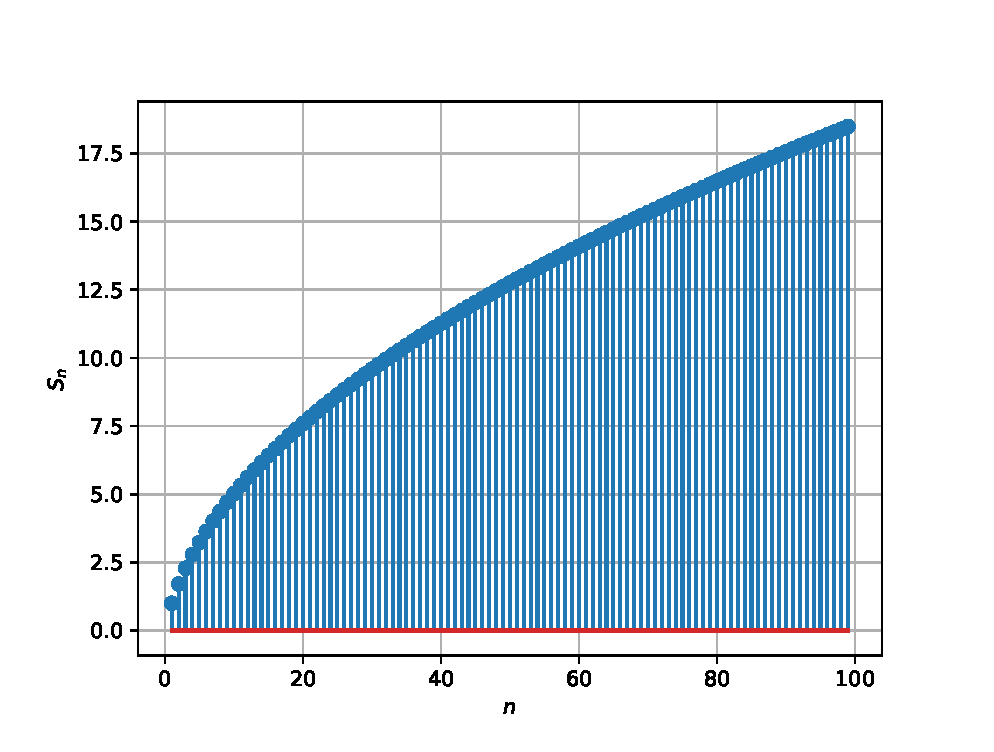
\includegraphics[width=\columnwidth]{./figs/8.eps}
\end{center}
\captionof{figure}{}
\label{fig:8}	
\end{figure}
Since
\begin{align}
\frac{1}{\sqrt{n}} > \frac{1}{n},
\end{align}
and $\sum \limits _{{n=1}}^{\infty}\,\frac{1}{n} $ diverges, from Proposition \ref{prop:inequality}, $\sum \limits _{{n=1}}^{\infty}\,\abs{u_n} $ diverges.  Hence $u_n$ 
is conditionally convergent.
\end{document}

